%!TEX root = thesis.tex

\chapter{Related Work}
\label{ch:relatedwork}

\todo{This won't go into }

\section{Pmariglia}
\label{sec:pmariglia}
The developer \textit{Pmariglia}\cite{Github:pmariglia-showdown} created a sophisticated
battling bot for Pokémon Showdown. This implementation is open source and can be found 
at \url{https://github.com/pmariglia/showdown}. On the repository, you can find two 
different approaches: \\

\paragraph{Safest}
The \textit{Safest} approach searches through the game-tree for two turns and selects the 
move that minimizes the possible loss for a turn. As Pokémon battles make heavy use of
\ac{RNG}, the author takes a weighted average for all possible end states. This is explained
in more detail in \todo{Link to section where we take miss chance into account}.

\paragraph{Nash-Equilibrium (experimental)}
In game theory, the \textit{Nash-Equilibrium} is the most common way to define a solution
of a non-cooperative game involving two or more players.  In a Nash equilibrium, each player 
is assumed to know the equilibrium strategies of the other players and no player has 
anything to gain by changing only their own strategy \cite{wiki:Nash_equilibrium}.

\section{Showdown AI Competition}
The authors of the \textit{Showdown AI Competition}\cite{Lee_Togelius_2017} compared many
simple AI implementations with each other. \todo{Does not describe how damage
is calculated}
\paragraph{Breath-first search}
\label{sec:showdown-competition-bfs}
Given a root battle object representing the current game state, \ac{BFS} explores the
outcomes of all possible choices, treating these resultant states as child nodes. This
algorithm traverses the game tree until it finds a state in which the enemy Pokémon is
fainted. As a non-adversarial algorithm, the agent assumes that the enemy does not 
move at all \cite{Lee_Togelius_2017}. 

\paragraph{Minimax}
This variant of the \textit{Minimax}-Algorithm deals with adversarial paradigms by assuming
that each player acts in their best interest. In this decision tree, each node represents
the worst case scenario that would occur as a result of the current choice. The agent
also uses alpha-beta pruning, ignoring any node in which the agents Pokémon faints. 
\todo{We take the average outcome. We don't prune fainting paths (explosion)}
The tree itself is traversed using a greedy strategy, which terminates under the same 
conditions as \ac{BFS}\ref{sec:showdown-competition-bfs}. Both the traversal order and 
worst-case evaluation are performed using the evaluation function \ref{eq:minmax-eval-func}
\cite{Lee_Togelius_2017}:
\begin{equation}
\label{eq:minmax-eval-func}
    Eval = \frac{\text{current hp}_{\text{Own Pokémonn}}}{\text{max hp}_{\text{Own Pokémonn}}} -
    3 \cdot \frac{\text{current hp}_{\text{Enemy Pokémonn}}}{\text{max hp}_{\text{Enemy Pokémonn}}} -
    0.3 \cdot \text{depth}
\end{equation}

\paragraph{One Turn Lookahead}
One Turn Lookahead is a heuristic based agent designed to encapsulate a greedy strategy that 
prioritizes damage output. The agent operates by estimating the damage dealt by all usable moves, 
including those usable by the agent's inactive but usble Pokemon. If the highest damaging move 
belongs to the active Pokemon, the agent will use that attack. If the most damaging move belongs to 
an inactive Pokemon, the agent will switch to that Pokemon \cite{Lee_Togelius_2017}.

\paragraph{Type Selector}
This is a variation of the \textit{One Turn Lookahead}-Agent that utilizes a short series of
if-else statements in its decision-making. At first, if the current Pokémon knows a move 
that drains the opponents \ac{HP} to zero, this move is selected. Otherwise, the 
favorability of the current matchup is evaluated. If the current type matchup is 
undesirable, the agent will switch to the Pokémon with an acceptable type matchup. If no
such Pokémon exists, the agent will default to the most damaging move 
\cite{Lee_Togelius_2017}.

\paragraph{Pruned Breadth-First Search}
This agent is designed to demonstrate a simple way to utilize domain knowledge as a cost-cutting 
measure. This algorithm does so by making modifications to the Breadth First Search agent. First, 
the algorithm does not simulate any actions that involve using a damaging move with a resisted type, 
nor does it simulate any actions that involve switching to a Pokemon with a subpar type matchup. 
Additionally, rather than selfishly assuming the opponent skips their turn in each simulation, the 
agent assumes its opponent is a One Turn Lookahead agent and simulates accordingly
\todo{This is copied word by word}\cite{Lee_Togelius_2017}.

\paragraph{Evaulation}
The authors demonstrated how very basic approaches already yield interesting results in the 
field of competitive Pokémon battles. As this thesis will demonstrate, simple approaches can 
yield even better results if more key-aspects of the game like \textit{Hazards} \todo{Link to Hazards},
\textit{Field Effects} \todo{Link to Field effects} and especially \textit{Status Effects}
\todo{Link to Status effects} and \textit{Stat Boosts} are taken into account. This thesis furthermore
introduces a variation of the \textit{Minmax}-Algorithm that allows for long term planning.

\section{Supervised Approach}
Summery of \cite{TheThirdBuild:PokemonAi}
\begin{itemize}
    \item Input features:
    \begin{itemize}
        \item Pokemon Attributes: Hp, Active, Status, Boosts
        \item Player side: Light screen, Hazards, voltaile (leech seed), last used move
        \item Battlefield: Weather, Pseudo-Weather, Terrain
    \end{itemize}
    \item Used Tensorflow
    \item 2.000.000 Training replays from Showdown Replays
    \item model
    \begin{itemize}
        \item Every turn of the battle treated as seperate example, answer: Which player wins. 81\% Win chance model accuracy
        \item Restructured: Would p1 win to what would p1 do next turn. 86\% Next switch in 93\% next move accuracy 88\% switching
        out or staying in. Does not say: Test / Training Data? Real Battles?
    \end{itemize}
    \item Future Turns:
    \begin{itemize}
        \item What move options are tehre
        \item What happens on all combinations
        \item Choose move that leads to the most winning combinations 
        \item Remove the less likely ones
    \end{itemize}
\end{itemize}

\section{Self-Play Policy Optimization Approach}
Researchers from \textit{New York University} \cite{Lee_Togelius_2017} were the first ones to apply
\textit{Q-Learning} to the field of Pokémon battles. Two agents using \textit{Q-Learning}
were developed: A single layer perceptron as well as a multi layer perceptron. Both agents were 
used to output the expected reward of all current moves and switches. Based on this, the best 
action was picked. Both agents were rewarded for defeating opponents Pokémon and punished for 
allowing one of its own Pokémon to faint. Because decisions made tend to have long term consequences, 
weights are updated using the last three (State, Action) pairs rather than the most recent pair only.
Additionally, in order to promote exploration, the agent employs an epsilon-greedy selection policy, 
causing it to randomly override its decision with a probability of 0.1. The single layer perceptron 
was trained using the Delta Rule, while the multilayer perceptron was trained using Delta Rule 
plus Backpropagation. The agent using a single layer perceptron won 90 out of 180 games against a
random agent whereas the multi layer perceptron won 86 out of 180 games. Due to the large amount
of \ac{RNG} in Pokémon games, more games would need to be played in order to confirm the superiority
of the single layer perceptron in this particular use case. \\

One year after the publication of \cite{Lee_Togelius_2017}, the authors of \cite{GottaTrainEmAll} 
improved this design. They used \ac{PPO} \cite{schulman2017proximal} to train an agent. They also
used embeddings to better represent a Pokémon. Data available at \cite{Kaggle:NewYorkData} was used
to create embeddings for each Pokémon. The Dataset contains stats of the first 721 Pokémon, each 
row contains the name, type(s), numerical stat data (such as \ac{HP}, \ac{ATK}, \ac{SPE}) and some other
data such as color, height and whether the Pokémon is considered legendary in game. To create
embeddings for each Pokémon, the data was turned into a graph to be used with Node2Vec 
\cite{grover2016node2vec} which creates embeddings from graph data in similar to
Word2Vec \cite{mikolov2013distributed}. This algorithm samples random walks of some number
of nodes of a given graph. Using these random walks, a skip-gram model is created which
can be trained to generate embeddings. The Pokémon graph consisted of the name, type(s),
numerical attributes (total stats, \ac{HP}, \ac{ATK}, \ac{DEF}, \ac{SPA}, \ac{SPD}, \ac{SPE})
as well as two special nodes, \textit{Legendary} and \textit{Mega}\footnote{Mega is a mechanic
not available in the latest version of the game}. Lastly, Node2Vec was applied to the graph.
\begin{table}[h]
    \centering
        \begin{tabular}{|l|p{0.7\textwidth}|}
            \hline
            Pokémon & Most similar Pokémon \\
            \hline
            \emph{Bulbasaur} & Chikorita, Turtwig, Nuzleaf, Petilil, Exeggucte, Skiploom, Jumpluff, Oddish, Budew \\
            \hline
            \emph{Caterpie} & Wurmple, Weedle, Kakuna, Metapod, Paras, Ledyba, Spinarak, Venonat, Silcoon \\
            \hline
            \emph{Mewto} & Lugia, Mesprit, Mew, Victini, Celebi, Cresselia, Volcation, \mbox{Ho-Oh}, Uxie \\
            \hline
        \end{tabular}
        \caption{Similar Pokémon within the embedding space of \cite{GottaTrainEmAll}}
        \label{tbl:Gotta-Embeddings}
\end{table}
Table \ref{tbl:Gotta-Embeddings} displays discovered similarity using this approach. Here, a similar Pokémon
to \textit{Mewtwo}, a \textit{Psychic}-Type, is \textit{Ho-Oh}, a \textit{Flying}-\textit{Fire}-Type. However,
these two have entirely different strengths and weaknesses. In addition to that, they don't share a single
move in their move set: 
In generation 6, \textit{Ho-Oh} has access to these moves: \textit{Aura Sphere}, \textit{Calm Mind}, 
\textit{Fire Blast}, \textit{Ice Beam}, \textit{Psystrike} and \textit{Recover} whereas \textit{Lugia}'s
move pool consists of \textit{Brave Bird}, \textit{Earthquake}, \textit{Flame Charge}, \textit{Roost},
\textit{Sacred Fire}, \textit{Substitute} and \textit{Toxic} \cite{DamageCalc:Gen6}. This inappropriate
classification is likely caused to both \textit{Pokémon} having similar stats and both being legendary.

Features are derived from the battle state in the simulator. At a high level, battles consist of two
sides. Each side consists of a team of Pokémon, and each Pokémon has some set of moves. Each of these 
objects (battle, side Pokémon, and move) has attributes that are used to derive a feature vector.
After experimenting with multiple network architectures, the authors settled on a three-layer 
fully connected neural network, each with 512 neurons and a ReLU activation function.

The authors of \cite{GottaTrainEmAll} trained the agent against a random agent, a default agent 
that always tries to pick a non-switching move as well as a minimax agent
until the reward curve stabilized which was around 100 epochs where an epoch is a single battle between
two players. A reward of $+1$ is given to the agent if it wins the battle, $-1$ if it loses the battle and
$0$ for all other cases. The average epoch reward after training convergence for this approach can
be found in table \ref{tbl:Gotta-Performance}
\begin{table}[h]
    \centering
        \begin{tabular}{|l|l|}
            \hline
            Opponent & Average epoch reward \\
            \hline
            \emph{Random} & $0.85$ \\
            \hline
            \emph{Default} & $0.85$ \\
            \hline
            \emph{Minmax} & $-0.9$ \\
            \hline
        \end{tabular}
        \caption{Average epoch rewards after training convergence for opponent agents \cite{GottaTrainEmAll}}
        \label{tbl:Gotta-Performance}
\end{table}
The authors of \cite{GottaTrainEmAll} describe their final agent as flawed as while the agent learned 
to switch Pokémon when the active Pokémon reaches low health, it almost always chooses to switch to the
Pokémon in the last slot. In addition, this agent preferentially chooses the fourth move. 

\subsection{State of the art}
In 2019, the authors of \cite{Huang_Lee_2019} published a paper titled \emph{A Self-Play Policy 
Optimization Approach to Battling Pokémon}. This paper will be summarized in more depth as it
is very detailed and the agents proposed are performing on par with the state-of-the-art
search based Pokémon Ai.\\
Similar to
OpenAI's Dota AI \cite{OpenAI_dota}, the agent is represented using an actor-critic neural network.
Actor-critic RL methods \todo{This is the same source as in the paper}\cite{Konda_Tsitsiklis}
combine policy-based and value-based RL methods by predicting both policy and value for a given 
state, and then using the value prediction, the \glqq critic\grqq, as an estimate of expected
return when updating the policy prediction, the \glqq actor\grqq. The authors represent both
actor and critic using a two-headed neural network which is trained via self-play RL
\cite{Huang_Lee_2019}.

\paragraph{Neural Network}
Input to the neural network is the current state of the game, from the point of view of the player,
represented as multi-level tree-like structure:
\begin{enumerate}
    \item The \textit{battle} consists of two \textit{teams}, along with weather effects.
    \item Each \textit{team} consists of six \textit{Pokémon}, along with side conditions 
    described in \todo{Link to side conditions}
    \item Each \textit{Pokémon} has many features. Table \ref{tbl:HuangLee-Pokemon-Table} contains a partial 
    list\footnote{The authors state that this list is not complete but no additional information is provided.}
\end{enumerate}
\begin{table}[h]
\centering
    \begin{tabular}{llll}
    \hline \\
    Feature             & Type        & Dims            & Description                 \\
    \hline \\
    \emph{species}      & categorical & $1 \times 1023$ & e.g. Pikachu                \\
    \emph{item}         & categorical & $1 \times 368$  & e.g. Leftovers, Choice Band  \\
    \emph{ability}      & categorical & $4 \times 238$  & e.g. Rough Skin, Shadow Tag \\
    \emph{moveset}      & categorical & $4 \times 731$  & e.g. Flamethrower, Surf     \\
    \emph{lastmove}     & categorical & $1 \times 731$  & The last move used          \\
    \emph{stats}        & continuous  & 6               & \ac{HP}, \ac{ATK}, \ac{DEF}, \ac{SPA}, \ac{SPD}, \ac{SPE} \\
    \emph{boosts}       & continuous  & 6               & Temporary boosts for stats \\
    \emph{hp}           & continuous  & 1               & Current number of \ac{HP} \\
    \emph{maxhp}        & continuous  & 1               & Number of \ac{HP} at full health \\
    \emph{ppUsed}       & continuous  & 4               & \# times a move was used \\
    \emph{active}       & indicator   & 1               & 1 if Pokémon is active, else 0 \\
    \emph{fainted}      & indicator   & 1               & 1 if Pokémon has no \ac{HP}, else 0 \\
    \emph{status}       & indicator   & 28              & e.g. \ac{SLP}, \ac{BRN}, \ac{PAR} \\
    \emph{types}        & indicator   & 18              & e.g. \textit{Bug}, \textit{Fire} \\
    \emph{volatiles}    & indicator   & 23              & e.g. Leech Seed, Perish Song
    \end{tabular}
    \caption{Features used to describe a single Pokémon battle \cite{Huang_Lee_2019}}
    \label{tbl:HuangLee-Pokemon-Table}
\end{table}
The network has two outputs: a probability distribution $\pi \in \mathbb{R}^n$ over actions to take, 
and an estimate of player strength in the current state $v \in \mathbb{R}$. The probability distribution
$\pi$ is computed as follows:
\begin{enumerate}
    \item The network outputs an intermediate vector $p \in \mathbb{R}^n$. Each of the colored cells in
    figure \ref{fig:lee-network} correspond to an element of $p$
    \item A probability distribution $\pi' \in \mathbb{R}^n$ is computed by using the
    softmax function: $\pi' = \frac{\exp(p_i)}{\sum_i \exp(p_i)}$
    \item As not every action is valid in every state, for example, a switch to a Pokémon is invalid
    if that Pokémon is already fainted, the authors ensure their agent has zero probability of taking
    invalid actions. To do this, they take a mask $s \in \{0, 1\}^n$ as part of the input, and 
    renormalize probabilities to obtain $\pi: \pi_i = \frac{s_i \pi'_i}{s^T \pi'}$
\end{enumerate}
\begin{figure}
	\centering
	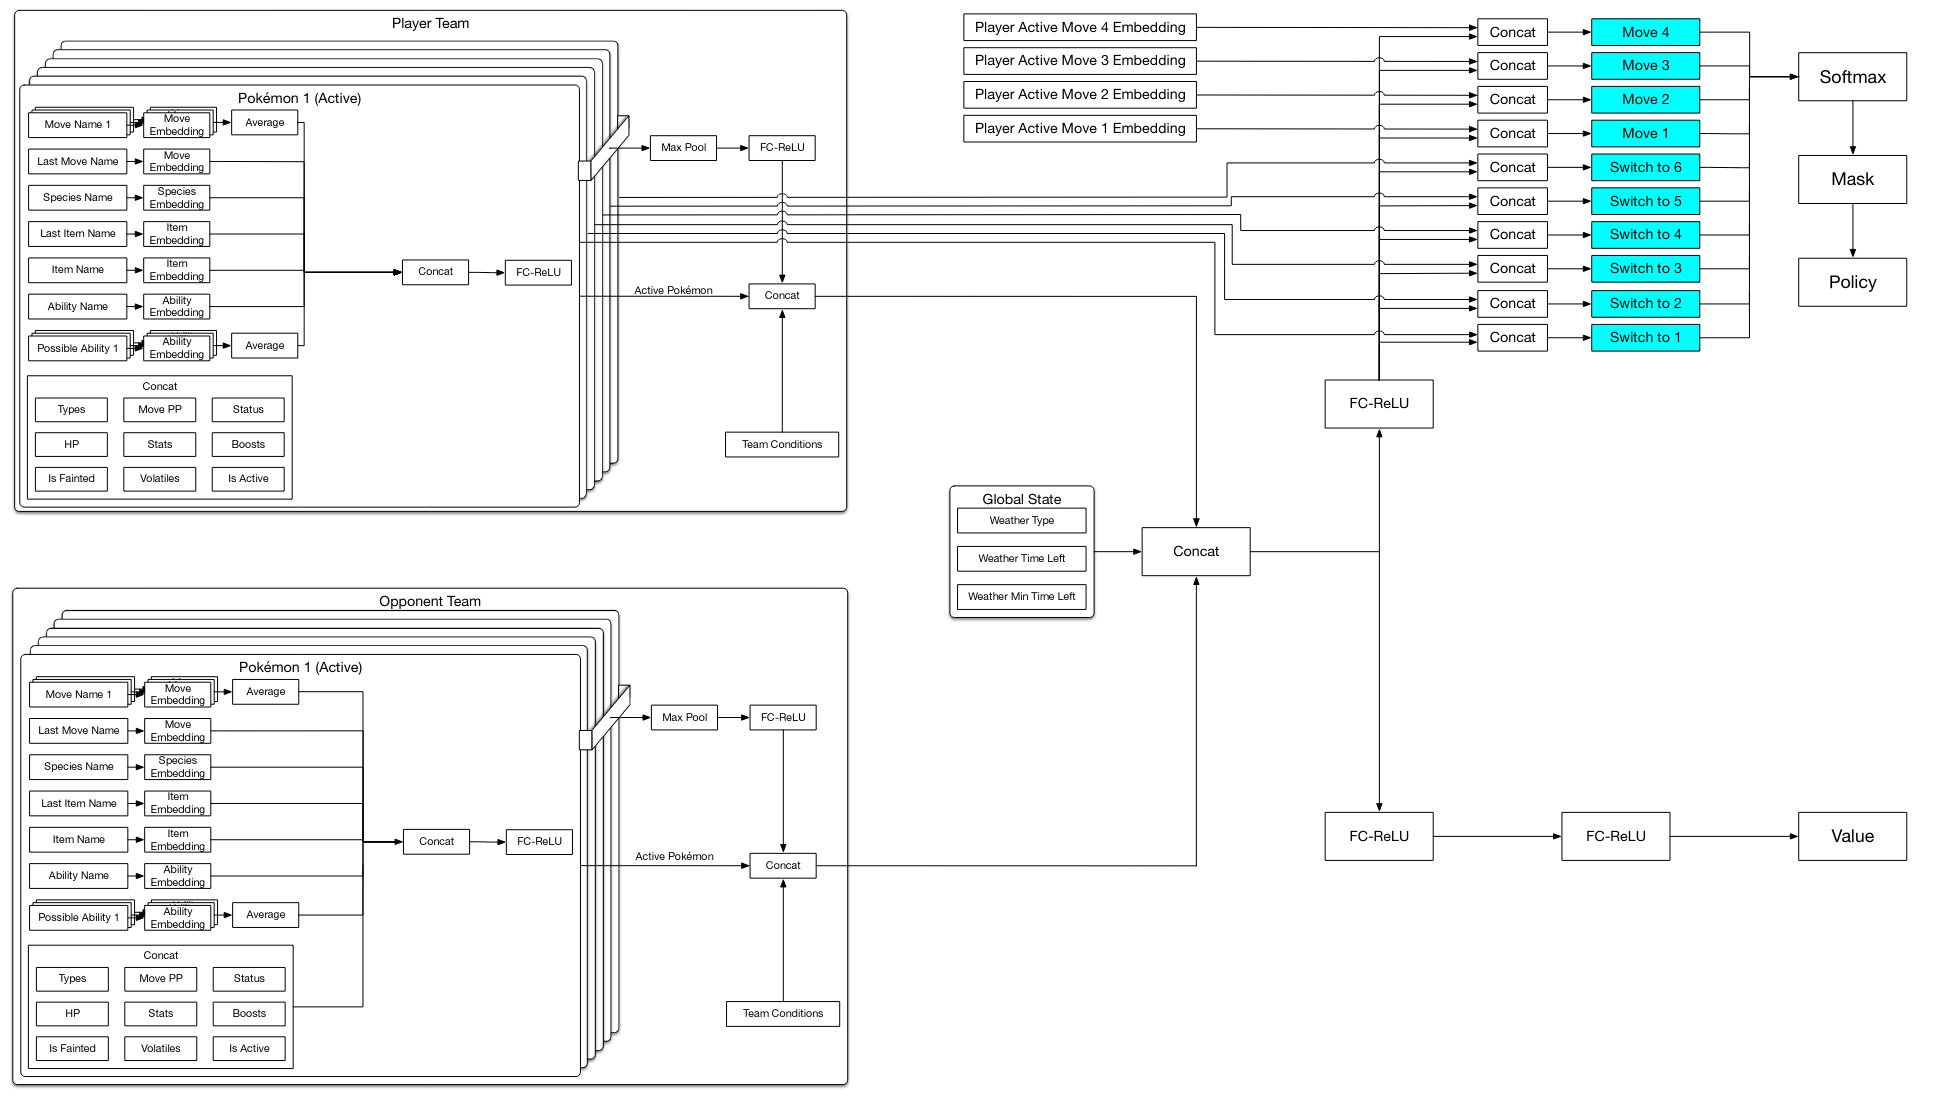
\includegraphics[width=0.9\textwidth]{images/RL-Network-Structure.png}
	\caption{The actor-critic neural network used by the authors in \cite{Huang_Lee_2019}}
	\label{fig:lee-network}
\end{figure}
The authors point out the following two key design decisions: First, a 128-dimensional entity embedding layer
for each of the categorical variables is used. This enables capturing similarities between different moves,
species and abilities without having to directly model their, often complicated, effects. Second, the
parameters for computing $p$ from above are shared among all $n$ actions. The resulting network is described
by figure \ref{fig:lee-network} and contains 1,327,618 parameters in total \cite{Huang_Lee_2019}.

\paragraph{Training the network}
Training was done serially: After $m = 7680$ games per iteration, the neural network parameters are updated
using the $2m$ self-play matches as training data to obtain new neural network parameters. A reward
of $+1$ for a win and $-1$ for a loss are assigned at the end of the match. To speed up learning, a 
dense reward signal using reward shaping was constructed. Auxiliary rewards are assigned based on
events that occur over the course of the match. For example, a reward of $-0.0125$ is added when a 
Pokémon of the agent faints, and a reward of $+0.0025$ whenever the player's Pokémon makes a 
super effective move. \\
To update the neural network, the authors use \textit{Proximal Policy Optimization}, which optimizes
an objective function that combines expected reward, accuracy of state value prediction, and a bonus
for high entropy policies. To reduce the variance of policy gradient estimates, \textit{Generalized
Advantage Estimation} is used \todo{Link Paper to both}. \\
After 500 iterations of the training loop, 3,840,000 self-play matches had been played by the neural
network. Training was performed using Google Cloud Platform over the course of 6 days with an 
approximated cost of \$91 USD.

\paragraph{Evaluation}
The refined embeddings as well as the complex network architecture lead to this agent outperforming
the RL-Agent described in \cite{GottaTrainEmAll}. Futhermore, the authors played 1.000 games against
the open source agent of \textit{pmariglia} described in \todo{Cite Chapter for search agents}.
\begin{table}[h]
    \centering
        \begin{tabular}{|l|l|l|}
            \hline
            \textbf{Opponent} & \textbf{Wins} & \textbf{Losses} \\
            \hline
            \emph{random} & 995 & 5 \\
            \hline
            \emph{max-damage} & 929 & 71 \\
            \hline
            \emph{max-damage-typed} & 829 & 171 \\
            \hline
            \emph{pmariglia} & 612 & 388 \\
            \hline
        \end{tabular}
        \caption{Performance of the agent developed by \cite{Huang_Lee_2019}}
        \label{tbl:State-Of-The-Art-Results}
\end{table} 
Table \ref{tbl:State-Of-The-Art-Results} describes the performance of the agent developed by
\cite{Huang_Lee_2019}